\begin{name}
	{GV biên soạn: Huỳnh Công Minh\\ GV phản biện 1: Nguyễn Liên Phúc Quỳnh}
	{TOÁN 10-KNTT-CS}
\end{name}

\setcounter{section}{26}
\section{Thực hành tính xác suất theo định nghĩa cổ điển}
%-------------------------------------------
\subsection{KIẾN THỨC TRỌNG TÂM}
\subsubsection{Sử dụng phương pháp tổ hợp}
\begin{dn}
Trong nhiều bài toán, để tính số phần tử không gian mẫu, của các biến cố, ta thường sử dụng các quy tắc đếm, các công thức tính số hoán vị, chỉnh hợp và tổ hợp.
\end{dn}
%\begin{dl}
%	content...
%\end{dl}
%\begin{tc}
%	content...
%\end{tc}
%\begin{nx}
%	content...
%\end{nx}
%\begin{hq}
%	content...
%\end{hq}
%\begin{chuy}
%	content...
%\end{chuy}
%-------------------------------------------
\subsubsection{Sử dụng sơ đồ cây}
\begin{dn}
Trong một số bài toán, phép thử $T$ được hình thành từ một vài phép thử, chẳng hạn: gieo xúc xắc liên tiếp bốn lần; lấy ba viên bi, mỗi viên từ một hộp;\ldots Khi đó ta sử dụng sơ đồ hình cây để có thể mô tả đầy đủ, trực quan không gian mẫu và biến cố cần tính xác suất.

\end{dn}
%\begin{dl}
%	content...
%\end{dl}
%\begin{tc}
%	content...
%\end{tc}
%\begin{nx}
%	content...
%\end{nx}
%\begin{hq}
%	content...
%\end{hq}
%\begin{chuy}
%	content...
%\end{chuy}
%-------------------------------------------
\subsubsection{Xác suất của biến cố đối}
\begin{dn}
Cho  $E$ là một biến cố. Xác suất của biến cố $\overline{E}$ liên hệ với xác suất của $E$ bởi công thức sau:
$$\mathrm{P}\left(\overline{E}\right)=1-\mathrm{P}\left(E\right).$$


\end{dn}


\subsection{PHÂN LOẠI VÀ PHƯƠNG PHÁP GIẢI TOÁN}


\begin{dang}[Tính xác suất theo định nghĩa cổ điển]
	\textbf{Phương pháp:} Ta có thể sử dụng các công thức sau
	\begin{itemize}
		\item Tính xác suất theo thống kê ta sử dụng công thức
		$$\mathrm{P} \left(A\right)=\dfrac{n}{N}.$$
		\item  Tính xác suất của biến cố theo định nghĩa cổ điển ta sử dụng công thức
		$$\mathrm{P} \left(A\right)=\dfrac{n\left(A\right)}{n \left(\Omega\right)}.$$
	\end{itemize}
\end{dang}

%%%=============vd_1=============%%%
\begin{vd}%[0D0N2-2]%[Biên soạn tài liệu dạy học bộ KNTT-CS]%[GV: Huỳnh Công Minh]
	Gieo một con xúc xắc cân đối đồng chất. Tính xác suất của biến cố \lq \lq Mặt có số chấm chẵn xuất hiện\rq \rq.
	\loigiai{Không gian mẫu $\Omega = \left\{1;2;3;4;5;6\right\}$ suy ra $n(\Omega)=6$.\\
		Gọi $A$ là biến cố: \lq \lq Mặt có số chấm chẵn xuất hiện\rq \rq. 
		\\
		Khi đó $A=\left\{2;4;6\right\}$ nên $n(A)=3$.\\
		Do đó $\mathrm{P}(A)=\dfrac{n(A)}{n(\Omega)}=\dfrac{1}{2}$.
	}
\end{vd}
%%%=============================%%%

%%%=============vd_2=============%%%
\begin{vd}%[0D0N2-2]%[Biên soạn tài liệu dạy học bộ KNTT-CS]%[GV: Huỳnh Công Minh]
	Gieo lần lượt hai con xúc xắc cân đối đồng chất. Tính xác suất của biến cố \lq \lq Số chấm xuất hiện trên mặt hai con xúc xắc giống nhau \rq \rq.
	\loigiai{Số phần tử của không gian mẫu là $n(\Omega)=6 \cdot 6=36$.\\
		Gọi $A$ là biến cố: \lq \lq Số chấm xuất hiện trên mặt hai con xúc xắc giống nhau\rq \rq.\\
		Có $6$ kết quả thuận lợi cho biến cố $A$ là $\left\{1;1\right\}$; $\left\{2;2\right\}$; $\left\{3;3\right\}$; $\left\{4;4\right\}$; $\left\{5;5\right\}$; $\left\{6;6\right\}$.\\
		Xác suất để số chấm xuất hiện trên mặt hai con xúc xắc giống nhau là $$\mathrm{P}(A)=\dfrac{n(A)}{n(\Omega)}=\dfrac{6}{36}=\dfrac{1}{6}.$$
	}
\end{vd}
%%%=============================%%%

%%%=============vd_3=============%%%
\begin{vd}%[0D0H2-2]%[Biên soạn tài liệu dạy học bộ KNTT-CS]%[GV: Huỳnh Công Minh]
	Gieo một con xúc xắc cân đối đồng chất $2$ lần, tính xác suất của biến cố \lq Tích số chấm ở $2$ lần khi gieo xúc xắc là một số chẵn\rq \rq.
	\loigiai{Số phần tử của không gian mẫu là $n(\Omega)=6 \cdot 6=36$.\\
		Gọi $A$ là biến cố: \lq \lq Tích hai lần số chấm khi gieo xúc xắc là một số chẵn \rq \rq.\\
		Ta xét các trường hợp sau:\\
		\textbf{Trường hợp 1:} Gieo lần một, số chấm xuất hiện trên mặt là số lẻ thì khi gieo lần hai, số chấm xuất hiện phải là số chẵn. Khi đó có $3 \cdot 3=9$ cách gieo.\\
		\textbf{Trường hợp 2}: Gieo lần một, số chấm xuất hiện trên mặt là số chẵn thì có hai trường hợp xảy ra là số chấm xuất hiện trên mặt khi gieo lần hai là số lẻ hoặc số chẵn. \\
		Khi đó có $3 \cdot 3+3 \cdot 3 =18$ cách gieo.\\
		Suy ra số kết quả thuận lợi cho biến cố là $n(A)=9+18=27$.\\
		Vậy xác suất cần tìm là $\mathrm{P}(A)=\dfrac{27}{36}=0{,}75$.
	}
\end{vd}
%%%=============================%%%

%%%=============vd_4=============%%%
\begin{vd}%[0D0H2-4]%[Biên soạn tài liệu dạy học bộ KNTT-CS]%[GV: Huỳnh Công Minh]
	Một nhóm học sinh gồm có $9$ nam, $3$ nữ. Tính xác suất để khi chọn ngẫu nhiên $4$ người thì có đúng $1$ nữ. 
	\loigiai{Số phần tử của không gian mẫu là $n(\Omega) = \mathrm{C}_{12}^{4}=495$.\\
		Gọi $A$ là biến cố: \lq \lq Trong $4$ người được chọn thì có đúng $1$ nữ \rq \rq. \\	
		Để chọn $4$ người có đúng $1$ nữ thì phải chọn $1$ nữ và $3$ nam có $\mathrm{C}_{3}^{1} \cdot \mathrm{C}_{9}^{3}=252$ cách.\\ Do đó $n(A)=252$.\\
		Vậy xác suất cần tìm là $\mathrm{P}(A)=\dfrac{n(A)}{n(\Omega)}=\dfrac{252}{495}=\dfrac{28}{55}$. 
	}
\end{vd}
%%%=============================%%%
%-----------------------------------------

\begin{dang}[Tính xác suất theo biến cố xung khắc, biến cố đối]
	\textbf{Phương pháp:} Sử dụng biến cố xung khắc, biến cố đối và áp dụng các công thức:
	\begin{itemize}
		\item Nếu $A$ và $B$ xung khắc thì $\mathrm{P}(A\cup B)=\mathrm{P}(A)+\mathrm{P}(B)$.
		\item $\mathrm{P}\left(\overline{A}\right)=1-\mathrm{P}\left(A\right)$.
	\end{itemize}
\end{dang}

%%%=============vd_1=============%%%
\begin{vd}%[1D9H2-3]%[Biên soạn tài liệu dạy học bộ KNTT-CS]%[GV: Huỳnh Công Minh]
	Hai xạ thủ mỗi người bắn một viên đạn vào bia. Xác suất bắn trúng vòng $10$ của xạ thủ thứ nhất và xạ thủ thứ hai lần lượt là $0{,}9$ và $0{,}8$. Tính xác suất để có ít nhất một xạ thủ bắn trúng vòng $10$.
	\loigiai{
			\textbf{Cách 1:}
		Ta gọi các biến cố\\
		$A$: \lq\lq Xạ thủ thứ nhất bắn trúng vòng $10$\rq\rq.\\
		$B$: \lq\lq Xạ thủ thứ hai bắn trúng vòng $10$\rq\rq.\\
		$C$: \lq\lq Ít nhất một xạ thủ bắn trúng vòng $10$\rq\rq.\\
		Khi đó $\mathrm{P}(A)=0{,}9\Rightarrow \mathrm{P}\left(\overline{A}\right)=0{,}1$, $P(B)=0{,}8\Rightarrow \mathrm{P}\left(\overline{B}\right)=0{,}2$.\\
		Vậy $C=A\overline{B}+\overline{A}B+AB\Rightarrow \mathrm{P}(C)=0{,}9\cdot 0{,}2+0{,}1\cdot 0{,}8+0{,}9\cdot 0{,}8=0{,}98$.\\
		\textbf{Cách 2:} $\overline{C}$ là biến cố \lq\lq Cả $2$ đều bắn không trúng vòng $10$\rq\rq.\\
		Suy ra $\overline{C}=\overline{A}\overline{B}\Rightarrow \mathrm{P}\left(\overline{C}\right)=\mathrm{P}\left(\overline{A}\right)\mathrm{P}\left(\overline{B}\right)=0{,}02$.\\
		Vậy xác suất cần tìm là $\mathrm{P}(C)=1-\mathrm{P}\left(\overline{C}\right)=0{,}98$.
	}
\end{vd}
%%%=============================%%%

%%%=============vd_2=============%%%
\begin{vd}%[1D9V2-3]%[Biên soạn tài liệu dạy học bộ KNTT-CS]%[GV: Huỳnh Công Minh]
	Cho mạch điện gồm $4$ bóng đèn, xác suất hỏng của mỗi bóng là $0{,}05$. Tính xác suất để khi cho dòng điện chạy qua mạch điện thì mạch điện sáng (có ít nhất một bóng sáng).
	\begin{center}
		\usetikzlibrary{circuits,circuits.ee.IEC}
		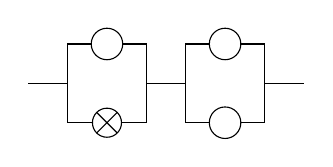
\begin{tikzpicture}[circuit ee IEC]
			\draw (0,0)--(0.5,0) (0.5,-0.5)--(0.5,0.5)--(1.5,0.5)--(1.5,-0.5) (0.5,-0.5) to[bulb] (1.5,-0.5);
			\draw (1.5,0)--(2,0) (2,-0.5)--(2,0.5)--(3,0.5)--(3,-0.5)--cycle (3,0)--(3.5,0);
			\draw[fill=white] (1,0.5) circle(0.2) (2.5,0.5) circle(0.2) (2.5,-0.5) circle(0.2);
		\end{tikzpicture}
	\end{center}
	\loigiai{
		Gọi $A_i$ là biến cố: \lq\lq Bóng đèn thứ $i$ sáng\rq\rq, với $i=\overline{1,4}$.\\
		Ta có các $A_i$ độc lập và $\mathrm{P}\left(A_i\right)=1-0{,}05=0{,}95$, $\mathrm{P}\left(\overline{A_i}\right)=0{,}05$.\\
		Gọi $A$ là biến cố: \lq\lq Có ít nhất một bóng đèn sáng\rq\rq.\\
		Để không có bóng đèn nào sáng ta có các trường hợp sau:
		\begin{itemize}
			\item \textbf{Trường hợp 1:} Cả $4$ bóng đèn cùng bị hỏng.\\
			$B$ là biến cố: \lq\lq Bốn bóng đèn bị hỏng\rq\rq.\\
			Khi đó xác suất để cả $4$ bóng đèn bị hỏng là $\mathrm{P}(B)=0{,}05^4=0{,}00000625$.
			\item \textbf{Trường hợp 2:} Ba bóng đèn bị hỏng.\\
			Gọi $C$ là biến cố: \lq\lq Ba bóng đèn bị hỏng\rq\rq.\\
			Xác suất để có $3$ bóng đèn bị hỏng là $\mathrm{P}(C)=4\cdot 0{,}05^3\cdot 0{,}95=0{,}000475$.
			\item \textbf{Trường hợp 3:} Hai bóng đèn phía trái hoặc hai bóng đèn phía phải bị hỏng.
			Gọi $D$ là biến cố: \lq\lq Hai bóng đèn phía trái hoặc hai bóng đèn phía phải bị hỏng\rq\rq.\\
			Xác suất để hai bóng đèn cùng phía bị hỏng là $\mathrm{P}(D)=2\cdot 0{,}05^2\cdot 0{,}95^2=0{,}0045125$.
		\end{itemize}
		Xác suất để có ít nhất một bóng đèn sáng là \[\mathrm{P}(A)=1-\left[\mathrm{P}(B)+\mathrm{P}(C)+\mathrm{P}(D)\right]=0{,}99500625.\]
	}
\end{vd}
%%%=============================%%%

%%%=============vd_3=============%%%
\begin{vd}%[1D9V2-3]%[Biên soạn tài liệu dạy học bộ KNTT-CS]%[GV: Huỳnh Công Minh]
	Một trường THPT có $18$ học sinh giỏi toàn diện, trong đó có $7$ học sinh khối $12$, $6$ học sinh khối $11$ và $5$ học sinh khối $10$. Chọn ngẫu nhiên $8$ học sinh từ $18$ học sinh trên để đi dự trại hè. Gọi $A$ là biến cố \lq\lq Mỗi khối có ít nhất $1$ học sinh được chọn\rq\rq.
	\begin{enumerate}
		\item Hãy tìm biến cố đối của biến cố $A$.
		\item Hãy tính xác suất của biến cố $A$.
	\end{enumerate}
	\loigiai{
		\begin{enumerate}
			\item Biến cố đối của biến cố $A$ là biến cố $\overline{A}$: \lq\lq $8$ học sinh được chọn thuộc cùng một khối hoặc thuộc hai khối\rq\rq.
			\item Chọn $8$ học sinh bất kì trong số $18$ học sinh, ta có số phần tử của không gian mẫu là $n(\Omega)=\mathrm{C}_{18}^8$\\
			Ta có $A$: \lq\lq Mỗi khối có ít nhất $1$ học sinh được chọn\rq\rq.\\
			Suy ra $\overline{A}$: \lq\lq $8$ học sinh được chọn thuộc cùng một khối hoặc thuộc hai khối\rq\rq.
			\begin{itemize}
				\item \textbf{Trường hợp 1:} Chọn $8$ học sinh không có khối $10$: $\mathrm{C}_{13}^8$.
				\item \textbf{Trường hợp 2:} Chọn $8$ học sinh không có khối $11$: $C_{12}^8$.
				\item \textbf{Trường hợp 3:} Chọn $8$ học sinh không có khối $12$: $C_{11}^8$.
			\end{itemize}
			Suy ra $n\left(\overline{A}\right)=\mathrm{C}_{13}^8+\mathrm{C}_{12}^8+\mathrm{C}_{11}^8$.\\
			Suy ra $\mathrm{P}\left(\overline{A}\right)=\dfrac{n\left(\overline{A}\right)}{n\left(\Omega\right)}=\dfrac{\mathrm{C}_{13}^8+\mathrm{C}_{12}^8+\mathrm{C}_{11}^8}{\mathrm{C}_{18}^8}=\dfrac{59}{1\,326}$.\\
			Vậy $\mathrm{P}(A)=1-\mathrm{P}\left(\overline{A}\right)=\dfrac{1\,267}{1\,326}$.
		\end{enumerate}
	}
\end{vd}
%%%=============================%%%

%%%=============vd_4=============%%%
\begin{vd}%[1D9H2-3]%[Biên soạn tài liệu dạy học bộ KNTT-CS]%[GV: Huỳnh Công Minh]
	Xét các số tự nhiên gồm $5$ chữ số khác nhau được lập từ các số $1$, $3$, $5$, $7$, $9$. Tính xác suất để tìm được một số không bắt đầu bởi $135$.
	\loigiai{
		Số tự nhiên gồm $5$ chữ số khác nhau được lập từ các số $1$, $3$, $5$, $7$, $9$ nên ta có số phần tử không gian mẫu là $n\left(\Omega\right)=5!=120$.\\
		Gọi biến cố $A$: \lq\lq Số tìm được không bắt đầu bởi $135$\rq\rq.\\
		Suy ra biến cố đối $\overline{A}$: \lq\lq Số tìm được bắt đầu bởi $135$\rq\rq.\\
		Giả sử, ta buộc $135$ lại xem như một phần tử thì ta còn lại $3$ phần tử là $135$, $7$, $9$.\\
		Suy ra $n\left(\overline{A}\right)=1\cdot 2\cdot 1=2$ cách nên $\mathrm{P}\left(\overline{A}\right)=\dfrac{2}{120}=\dfrac{1}{60}$ .\\
		Vậy $\mathrm{P}(A)=1-\dfrac{1}{60}=\dfrac{50}{60}$.
	}
\end{vd}
%%%=============================%%%

%-------------------------------------------
\subsection{BÀI TẬP RÈN LUYỆN}
%-------------Trắc nghiệm nhiều lựa chọn
\ind{PHẦN I.} \inden{Câu trắc nghiệm nhiều phương án lựa chọn. Mỗi câu hỏi học sinh chỉ chọn một phương án.}
\setcounter{ex}{0}
\Opensolutionfile{ans}[ans/ans-c8b27-lc]
%\begin{ex}%[ID]%[Biên soạn tài liệu dạy học bộ KNTT-CS]%[GV biên soạn]
%	
%	\choice
%	{\True }
%	{}
%	{}
%	{}
%	\loigiai{
%		
%	}
%\end{ex}

%Phần trắc nghiệm 1 phương án đúng

\Opensolutionfile{ans}[Ans/TamPAEX]
%%%=========EX_1=========%%%
\begin{ex}%[0D0N2-9]%[Biên soạn tài liệu dạy học bộ KNTT-CS]%[GV Huỳnh Công Minh]
	Trong không gian cho $10$ điểm, trong đó có $A$ và $B$, sao cho không có ba điểm nào thẳng hàng. Quỳnh vẽ một đoạn thẳng nối hai điểm tùy ý trong $10$ điểm. Tính xác suất để đoạn thẳng mà Quỳnh vẽ là đoạn $AB$.
	\choice
	{$\dfrac{1}{10}$}
	{$\dfrac{1}{90}$}
	{$\dfrac{1}{5}$}
	{\True $\dfrac{1}{45}$}
	\loigiai{
		Tổng số đoạn thẳng có thể vẽ là $\mathrm{C}_{10}^2 = 45$.\\
		Chỉ có duy nhất $1$ đoạn là $AB$ Nên $\mathrm{P}(A) = \dfrac{1}{45}$.
	}
\end{ex}

%%%=========EX_2=========%%%
\begin{ex}%[0D0N2-9]%[Biên soạn tài liệu dạy học bộ KNTT-CS]%[GV Huỳnh Công Minh]
	Chọn ngẫu nhiên một quân bài trong bộ bài tú lơ khơ gồm $52$ lá. Tính xác suất để quân bài được chọn có số nút là $9$.
	\choice
	{\True $\dfrac{1}{13}$}
	{$\dfrac{1}{12}$}
	{$\dfrac{1}{11}$}
	{$\dfrac{1}{10}$}
	\loigiai{
		Số phần tử của không gian mẫu là $n(\Omega) = \mathrm{C}_{52}^1 = 52$.\\
		Gọi $A$ là biến cố \lq\lq Quân bài được chọn có số nút là $9$\rq\rq.\\
		Mỗi giá trị nút có $4$ quân bài $\Rightarrow n(A) = 4$ Nên$ \mathrm{P}(A) = \dfrac{4}{52} = \dfrac{1}{13}$.
	}
\end{ex}

%%%=========EX_3=========%%%
\begin{ex}%[0D0N2-9]%[Biên soạn tài liệu dạy học bộ KNTT-CS]%[GV Huỳnh Công Minh]
	Từ một đội văn nghệ gồm $5$ nam và $8$ nữ cần lập một nhóm gồm $4$ người hát tốp ca. Xác suất để trong $4$ người được chọn đều là nam bằng
	\choice
	{$\dfrac{\mathrm{C}_8^4}{\mathrm{C}_{13}^4}$}
	{$\dfrac{\mathrm{A}_5^4}{\mathrm{C}_8^4}$}
	{\True $\dfrac{\mathrm{C}_5^4}{\mathrm{C}_{13}^4}$}
	{$\dfrac{\mathrm{C}_8^4}{\mathrm{A}_{13}^4}$}
	\loigiai{
		Tổng số cách chọn $4$ người từ $13$ người $n(\Omega) = \mathrm{C}_{13}^4$.\\
		Gọi $A$ là biến cố \lq\lq Chọn được $4$ người đều là nam\rq\rq.\\
		Vì có $5$ nam. Nên  $n(A) = \mathrm{C}_5^4$.\\
		Vậy xác suất của biến cố $A$ là $\mathrm{P}(A) = \dfrac{\mathrm{C}_5^4}{\mathrm{C}_{13}^4}$.
	}
\end{ex}

%%%=========EX_4=========%%%
\begin{ex}%[0D0N2-2]%[Biên soạn tài liệu dạy học bộ KNTT-CS]%[GV Huỳnh Công Minh]
	Từ một hộp chứa $5$ quả cầu trắng và $3$ quả cầu đen, lấy ngẫu nhiên $2$ quả. Xác suất để lấy được cả hai quả trắng là
	\choice
	{\True $\dfrac{5}{14}$}
	{$\dfrac{5}{28}$}
	{$\dfrac{10}{56}$}
	{$\dfrac{20}{28}$}
	\loigiai{
		Tổng số quả là $5 + 3 = 8$.\\
		Số cách chọn $2$ quả bất kỳ là $\mathrm{C}^2_8 = 28$. Do đó số phần tử của không gian mẫu là $ n(\Omega)=28$.\\
		Gọi $A$ là biến cố \lq\lq Lấy được hai quả cầu trắng\rq\rq.\\
		Số cách chọn $2$ quả trắng là $\mathrm{C}^2_5 = 10\Rightarrow n(A)=10$.\\
		Vậy xác suất của biến cố $A$ là
		\[
		\mathrm{P}(A) = \dfrac{10}{28} = \dfrac{5}{14}.
		\]		
	}
\end{ex}

%%%=========EX_5=========%%%
\begin{ex}%[0D0H2-1]%[Biên soạn tài liệu dạy học bộ KNTT-CS]%[GV Huỳnh Công Minh]
	Tung một đồng xu cân đối và đồng chất hai lần liên tiếp. Tính xác suất để cả hai lần tung đều xuất hiện mặt ngửa.
	\choice
	{ $\dfrac{1}{2}$ }
	{ $\dfrac{1}{3}$ }
	{\True $\dfrac{1}{4}$ }
	{ $\dfrac{3}{4}$ }
	\loigiai{
		Không gian mẫu của phép thử là $\Omega = \{SS,\ SN,\ NS,\ NN \}$.\\
		Xét biến cố $A$: \lq\lq Hai lần tung đều xuất hiện mặt ngửa\rq\rq. Nên $ A = \{NN\}$.\\
		Khi đó
		\[
		n(\Omega) = 4,\quad n(A) = 1,\quad \mathrm{P}(A) = \dfrac{n(A)}{n(\Omega)} = \dfrac{1}{4}.
		\]
	}
\end{ex}

%%%=========EX_6=========%%%
\begin{ex}%[0D0H2-1]%[Biên soạn tài liệu dạy học bộ KNTT-CS]%[GV Huỳnh Công Minh]
	Một bộ bài tú lơ khơ gồm $52$ quân. Lấy ngẫu nhiên $2$ quân bài. Xác suất lấy được $2$ quân át bằng
	\choice
	{\True $\dfrac{1}{121}$}
	{$\dfrac{2}{663}$}
	{$\dfrac{1}{1326}$}
	{$\dfrac{1}{26}$}
	\loigiai{
		Số phần tử của không gian mẫu là số cách chọn $2$ lá từ $52$ lá
		\[
		n(\Omega) = \mathrm{C}^2_{52}.
		\]
		Biến cố $A$: \lq\lq Lấy được $2$ quân át\rq\rq. Nên $ n(A) = \mathrm{C}^2_4$.\\
		Vậy xác suất là
		\[
		\mathrm{P}(A) = \dfrac{\mathrm{C}^2_4}{\mathrm{C}^2_{52}} = \dfrac{6}{1326} = \dfrac{1}{121}.
		\]
		
	}
\end{ex}

%%%=========EX_7=========%%%
\begin{ex}%[0D0H2-1]%[Biên soạn tài liệu dạy học bộ KNTT-CS]%[GV Huỳnh Công Minh]
	Tung một đồng xu cân đối và đồng chất ba lần liên tiếp. Tính xác suất để có ít nhất một lần tung xuất hiện mặt sấp.
	\choice
	{$\dfrac{1}{8}$}
	{\True $\dfrac{7}{8}$}
	{$\dfrac{1}{4}$}
	{$\dfrac{3}{4}$}
	\loigiai{
		Số phần tử của không gian mẫu là $\quad n(\Omega) = 2\cdot 2\cdot 2= 8$.\\
		Xét biến cố $A$: \lq\lq Ít nhất một lần tung xuất hiện mặt sấp\rq\rq.\\
		Biến cố đối của $A$ là \lq\lq Không có lần nào sấp\rq\rq \ tức là chỉ có kết quả $\mathrm{NNN}$, nên $n(A)=8-1=7$.\\
		Vậy xác suất cần tìm là
		\[
		\mathrm{P}(A) = \dfrac{n(A)}{n(\Omega)} = \dfrac{7}{8}.
		\]
	}
\end{ex}

%%%=========EX_8=========%%%
\begin{ex}%[0D0H2-1]%[Biên soạn tài liệu dạy học bộ KNTT-CS]%[GV Huỳnh Công Minh]
	Một em bé có bộ $6$ thẻ chữ, trên mỗi thẻ có ghi một chữ cái, trong đó có $3$ thẻ chữ T, một thẻ chữ N, một thẻ chữ H và một thẻ chữ P. Em bé đó xếp ngẫu nhiên $6$ thẻ đó thành một hàng ngang. Tính xác suất em bé xếp được thành dãy \textbf{TNTHPT}.
	\choice
	{\True $\dfrac{1}{120}$}
	{$\dfrac{1}{720}$}
	{$\dfrac{1}{6}$}
	{$\dfrac{1}{20}$}
	\loigiai{
		Xem ba chữ T là phân biệt ta có $n(\Omega) = 6!$.\\
		Gọi $A$ là biến cố \lq\lq xếp ngẫu nhiên $6$ thẻ đó thành dãy \textbf{TNTHPT} \rq\rq.\\
		Suy ra $n(A) = 3!$ (vì hoán vị các chữ T, còn N, H, P cố định).\\
		Vậy xác suất biến cố $A$ là $P(A) = \dfrac{3!}{6!} = \dfrac{1}{120}$.
	}
\end{ex}

%%%=========EX_9=========%%%
\begin{ex}%[0D0H2-2]%[Biên soạn tài liệu dạy học bộ KNTT-CS]%[GV Huỳnh Công Minh]
	Gieo một con xúc xắc ba lần liên tiếp. Xác suất để mặt hai chấm xuất hiện cả ba lần là
	\choice
	{\True $\dfrac{1}{216}$}
	{$\dfrac{1}{72}$}
	{$\dfrac{1}{18}$}
	{$\dfrac{1}{20}$}
	\loigiai{
		Không gian mẫu là tập các bộ ba số $(i, j, k)$ với $i,j,k \in \{1,2,3,4,5,6\}$, nên
		$
		n(\Omega) = 6 \cdot 6 \cdot 6 = 216$.\\
		Biến cố $A$: \lq\lq Cả ba lần đều xuất hiện mặt $2$ chấm\rq\rq, chỉ có $1$ kết quả thuận lợi là $(2,2,2)$, nên $n(A) = 1$.\\
		Vậy xác suất cần tìm là
		$
		\mathrm{P}(A) = \dfrac{1}{216}$.
	}
\end{ex}

%%%=========EX_10=========%%%
\begin{ex}%[0D0H2-2]%[Biên soạn tài liệu dạy học bộ KNTT-CS]%[GV Huỳnh Công Minh]
	Gieo hai con xúc xắc. Tính xác suất của biến cố \lq\lq Tổng số chấm trên hai mặt là số lẻ\rq\rq.
	\choice
	{$\dfrac{11}{36}$}
	{\True $\dfrac{1}{2}$}
	{$\dfrac{1}{3}$}
	{$\dfrac{1}{4}$}
	\loigiai{
		Không gian mẫu là các bộ $(i, j)$ với $i,j \in \{1,2,3,4,5,6\}$.
		\[
		n(\Omega) = 6 \cdot 6 = 36.
		\]
		Gọi $A$ là biến cố \lq\lq Tổng số chấm trên hai mặt là số lẻ\rq\rq.\\
		\textbf{Trường hợp 1:} Xúc xắc thứ nhất ra số lẻ ($3$ cách), xúc xắc thứ hai ra số chẵn ($3$ cách) $\Rightarrow 3 \cdot  3 = 9$ cách.\\
		\textbf{Trường hợp 2:} Xúc xắc thứ nhất ra số chẵn ($3$ cách), xúc xắc thứ hai ra số lẻ ($3$ cách) $\Rightarrow 3 \cdot 3 = 9$ cách.\\
		$\Rightarrow n(A) = 9 + 9 = 18\Rightarrow 
		\mathrm{P}(A) = \dfrac{18}{36} = \dfrac{1}{2}$.
		
	}
\end{ex}


%%%=========EX_11=========%%%
\begin{ex}%[0D0H2-4]%[Biên soạn tài liệu dạy học bộ KNTT-CS]%[GV Huỳnh Công Minh]
	Ban chấp hành Đoàn thanh niên của nhà trường cần lập $4$ đội cờ đỏ để chấm thi đua, mỗi đội $3$ người từ $12$ học sinh gồm $5$ học sinh lớp $12$, $4$ học sinh lớp $11$, $3$ học sinh lớp $10$. Xác suất để đội nào cũng có học sinh lớp $12$ và học sinh lớp $11$ là
	\choice
	{\True $\dfrac{36}{385}$}
	{$\dfrac{6}{385}$}
	{$\dfrac{3}{770}$}
	{$\dfrac{9}{385}$}
	\loigiai{
		Số cách chia $12$ học sinh thành $4$ đội là 
		$n\left(\Omega\right)=\mathrm{C}_{12}^3\cdot\mathrm{C}_9^3\cdot\mathrm{C}_6^3\cdot\mathrm{C}_3^3$.\\
		Gọi $A$ là biến cố \lq\lq Mỗi đội luôn có học sinh lớp $12$ và học sinh lớp $11$\rq\rq.\\
		Xếp vào mỗi đội một học sinh lớp $11$ ta có $4!$ cách.\\
		Xếp $5$ học sinh lớp $12$ vào $4$ đội thì sẽ có $1$ đội có $2$ học sinh lớp $12$.\\
		Chọn đội có $2$ học sinh lớp $12$ có $4$ cách, chọn $2$ học sinh lớp $12$ có $ \mathrm{C}_5^2$ cách, xếp $3$ học sinh lớp $12$ còn lại có $3!$ cách.\\
		Xếp $3$ học sinh lớp $10$ có $3!$ cách.\\
		Ta có $ n(A)=4!\cdot4\cdot\mathrm{C}_5^2\cdot3!\cdot3!$.\\
		Xác suất của biến cố $A$ là $ \mathrm{P}(A)=\dfrac{4!\cdot4\cdot\mathrm{C}_5^2\cdot3!\cdot3!}{\mathrm{C}_{12}^3\cdot\mathrm{C}_9^3\cdot\mathrm{C}_6^3\cdot\mathrm{C}_3^3}=\dfrac{36}{385}$.
	}
\end{ex}

%%%=========EX_12=========%%%
\begin{ex}%[0D0V2-7]%[Biên soạn tài liệu dạy học bộ KNTT-CS]%[GV Huỳnh Công Minh]
	Gọi $S$ là tập hợp tất cả các số có $5$ chữ số khác nhau được lập từ các chữ số $0, 1, 2, 3, 4, 5, 6, 7$. Chọn ngẫu nhiên một số từ $S$. Tính xác suất để số chọn được chia hết cho $5$, luôn có mặt các chữ số $2, 3, 4$ và chúng đứng cạnh nhau.
	\choice
	{$\dfrac{1}{140}$}
	{$\dfrac{1}{392}$}
	{$\dfrac{4}{245}$}
	{\True $\dfrac{3}{196}$}
	\loigiai{
		Gọi số cần tìm là $\overline{abcde}$. Trong đó các chữ số $a, b, c, d, e$ đôi một khác nhau và thuộc tập hợp $M=\{0, 1, 2, 3, 4, 5, 6, 7 \}$, $a\ne 0$.\\
		Số các chữ số có $5$ chữ số đôi một khác nhau thuộc tập hợp $M$ là $n\left(\Omega\right)= 7\cdot\mathrm{A}_7^4=5\,880$.\\
		Gọi $A$ là biến cố \lq\lq số chọn được chia hết cho $5$, luôn có mặt các chữ số $2, 3, 4$ và chúng đứng cạnh nhau\rq\rq.\\
		Vì $\overline{abcde}\vdots 5$ nên $e\in\{0, 5\}$.\\
		Vì các chữ số $2, 3, 4$ luôn có mặt và chúng đứng cạnh nhau nên xếp $3$ ba chữ số $2, 3, 4$ thành một nhóm $(234)$ có $3!$ cách xếp.
		\begin{itemize}
			\item {\bf Trường hợp 1:} $e=0$.\\
				\begin{itemize}
			\item 	Xếp chữ số $e$ có $1$ cách.
				\item Xếp nhóm các chữ số $(234)$  có $2\cdot3!=12$ cách.
			\item 	Xếp các chữ số $1, 5, 6, 7$ vào vị trí còn lại có $4$ cách.
				\end{itemize}
			Vậy có  $12\cdot4=48$  cách.
			\item {\bf Trường hợp 2:} $e=5$.
			\begin{itemize}
				\item Xếp nhóm các chữ số $(234)$  vào vị trí $(abc)$ có $3!=6$ cách.\\
				Xếp các chữ số $0, 1, 6, 7$ vào vị trí $d$ có $4$ các xếp.\\
				Trường hợp này có $6\cdot4=24$ cách.
				\item Xếp nhóm các chữ số $(234)$  vào vị trí $(bcd)$ có $3!=6$ cách.\\
				Xếp các chữ số $1, 6, 7$ vào vị trí $a$ có $3$ các xếp.\\
				Trường hợp này có $6\cdot3=18$ cách.
			\end{itemize}
			Vậy có $24 + 18 = 42$ cách.
		\end{itemize}
		Do đó số kết quả thuận lợi của biến cố $A$ là $n\left(A\right)= 48+42 = 90$.\\
		Xác suất của biến cố $A$ là 
		$\mathrm{P}(A)=\dfrac{n(A)}{n\left(\Omega\right)}=\dfrac{90}{5\,880}=\dfrac{3}{196}$.
	}
\end{ex}
\Closesolutionfile{ans}
\Closesolutionfile{ans}
\indapan{6}{ans/ans-c8b27-lc}
%---------------------Trắc nghiệm đúng sai
\ind{PHẦN II.} \inden{Câu trắc nghiệm đúng sai. Trong mỗi ý a), b), c), d) ở mỗi câu, học sinh chọn đúng hoặc sai.}
\setcounter{ex}{0}
\Opensolutionfile{ans}[ans/ans-c8b27-ds]

\begin{ex}%[0D0H2-5]%[Biên soạn tài liệu dạy học bộ KNTT-CS]%[GV Huỳnh Công Minh]
	Có $100$ tấm thẻ được đánh số từ $1$ đến $100$. Lấy ngẫu nhiên $5$ thẻ. Khi đó
	\choiceTF
	{\True Số phần tử của không gian mẫu là $\mathrm{C}_{100}^5$}
	{Xác suất để $5$ thẻ lấy ra đều mang số chẵn là $0{,}5$}
	{\True Xác suất để $5$ thẻ lấy ra có $2$ thẻ mang số chẵn và $3$ thẻ mang số lẻ xấp xỉ bằng $ 0{,}32$}
	{Xác suất để có ít nhất một số ghi trên thẻ được chọn chia hết cho $3$ xấp xỉ bằng $0{,}78$}
	\loigiai{
		\begin{itemchoice}
			\itemch
			Vì lấy ngẫu nhiên $5$ thẻ từ $100$ thẻ nên số phần tử của không gian mẫu $ n\left(\Omega\right)=\mathrm{C}_{100}^5$.
			\itemch
			Gọi $A$ là biến cố \lq\lq $5$ thẻ lấy ra đều mang số chẵn\rq\rq.\\
			Vì từ $1$ đến $100$ có $50$ số chẵn, suy ra số cách chọn $5$ thẻ đều mang số chẵn là $n(A)=\mathrm{C}_{50}^5.$\\
			Vậy xác suất để $5$ thẻ lấy ra đều mang số chẵn là 
			$$ \mathrm{P}(A)=\dfrac{n(A)}{n\left(\Omega\right)}
			=\dfrac{\mathrm{C}_{50}^5}{\mathrm{C}_{100}^5}\approx 0{,}028 \ne 0{,}5.$$
			\itemch
			Gọi $B$ là biến cố \lq\lq $5$ thẻ lấy ra có $2$ thẻ mang số chẵn và $3$ thẻ mang số lẻ\rq\rq.\\
			Suy ra $n(B)=\mathrm{C}_{50}^2\cdot\mathrm{C}_{50}^3$.\\
			Vậy $\mathrm{P}(B)=\dfrac{n(B)}{n\left(\Omega\right)}
			=\dfrac{\mathrm{C}_{50}^2\cdot\mathrm{C}_{50}^3}{\mathrm{C}_{100}^5}\approx 0{,}32$.
			\itemch
			Gọi $C$ là biến cố \lq\lq Ít nhất một số ghi trên $5$ thẻ được chọn chia hết cho $3$\rq\rq.\\
			Suy ra $\overline{C}\colon$ \lq\lq Cả $5$ số trên $5$ thẻ được chọn đều không chia hết cho $3$\rq\rq.\\
			Vì từ $1$ đến $100$ có $67$ số không chia hết cho $3$, suy ra số cách chọn $5$ thẻ đều đều không chia hết cho $3$ là $ n\left(\overline{C}\right)=\mathrm{C}_{67}^5$.\\
			Vậy $ \mathrm{P}(C)=\dfrac{n(C)}{n\left(\Omega\right)}=\dfrac{\mathrm{C}_{100}^5-\mathrm{C}_{67}^5}{\mathrm{C}_{100}^5}\approx 0{,}87\ne 0{,}78$.
		\end{itemchoice}
	}
\end{ex}

%%%=========TF_2=========%%%
\begin{ex}%[0D0H2-5]%[Biên soạn tài liệu dạy học bộ KNTT-CS]%[GV Huỳnh Công Minh]
	Một hộp có $5$ viên bi xanh, $6$ viên bi đỏ và $7$ viên bi vàng. Xét phép thử chọn ngẫu nhiên $3$ viên bi. Khi đó
	\choiceTF
	{\True Số phần tử của gian mẫu của phép thử là $816$}
	{Xác xuất để chọn được $3$ viên bi đỏ là $\dfrac{1}{272}$}
	{\True Xác xuất để chọn được $3$ viên bi có đủ $3$ màu là $\dfrac{35}{136}$}
	{\True Xác xuất chọn được nhiều nhất $2$ viên bi xanh là $\dfrac{403}{408}$}
	\loigiai{
		\begin{itemchoice}
			\itemch
			Vì chọn $2$ viên bi trong $5+6+7=18$ viên bi nên số phần tử gian mẫu của phép thử là $n\left(\Omega\right)=\mathrm{C}_{18}^3= 816$. 
			\itemch
			Gọi $A$ là biến cố \lq\lq chọn được $3$ viên bi đỏ\rq\rq.\\
			Suy ra $n(A)=\mathrm{C}_{6}^3= 20$.\\
			Vậy xác suất để chọn được $3$ viên bi đỏ là 
			$\mathrm{P}(A)=\dfrac{n(A)}{n\left(\Omega\right)}
			=\dfrac{20}{816}=\dfrac{5}{204}\ne \dfrac{1}{272}$.
			\itemch
			Gọi $B$ là biến cố \lq\lq chọn được $3$ viên bi có đủ $3$ màu\rq\rq.\\
			Suy ra $n(B)=\mathrm{C}_{5}^1\cdot\mathrm{C}_{6}^1\cdot\mathrm{C}_{7}^1= 210$.\\
			Vậy xác suất để chọn được $3$ viên có đủ $3$ màu là 
			$\mathrm{P}(B)=\dfrac{n(B)}{n\left(\Omega\right)}
			=\dfrac{210}{816}=\dfrac{35}{216}$.
			\itemch
			Gọi $C$ là biến cố \lq\lq chọn được nhiều nhất $2$ viên bi xanh\rq\rq.\\
			Suy ra $\overline{C}\colon$ \lq\lq chọn được $3$  viên bi xanh\rq\rq.\\
			Suy ra $n\left(\overline{C}\right)=\mathrm{C}_{5}^3=10$.
			Vậy $ \mathrm{P}(C)=1-\mathrm{P}\left(\overline{C}\right)=1-\dfrac{10}{816}=\dfrac{403}{408}$.
		\end{itemchoice}
		
	}
\end{ex}

%%%=========TF_3=========%%%
\begin{ex}%[0D0H2-2]%[Biên soạn tài liệu dạy học bộ KNTT-CS]%[GV Huỳnh Công Minh]
	Gieo một đồng xu cân đối liên tiếp $4$ lần. Kí hiệu $S$ và $N$ tương ứng là đồng xu ra mặt sấp và đồng xu ra mặt ngửa. Khi đó
	\choiceTF
	{Biến cố $A$: \lq\lq Cả $4$ lần gieo đều xuất hiện mặt ngửa\rq\rq\ là biến cố không thể}
	{Biến cố $B$: \lq\lq Có ít nhất một lần gieo xuất hiện mặt sấp\rq\rq\ là biến cố chắc chắn}
	{\True Xác suất của biến cố $C$: \lq\lq Có đúng một lần gieo xuất hiện mặt sấp\rq\rq\ là $\mathrm{P}(C)=\dfrac{1}{4}$}
	{\True Xác suất của biến cố $D$: \lq\lq Có hai lần gieo xuất hiện mặt sấp và hai lần gieo xuất hiện mặt ngửa\rq\rq\ là $\mathrm{P}(D)=\dfrac{3}{8}$}
	\loigiai{
		\begin{itemchoice}
			\itemch Ta có $A=\{NNNN\}$ nên $A$ không là biến cố không thể.
			\itemch Ta có trường hợp \lq\lq $NNNN$\rq\rq\ thuộc không gian mẫu nhưng không thuộc $B$ nên $B$ không là biến cố chắc chắn.
			\itemch Số phần tử của không gian mẫu là $16$.\\
			Có $C=\{SNNN; NSNN; NNSN; NNNS\}$ nên $\mathrm{P}(C)=\dfrac{4}{16}=\dfrac{1}{4}$.
			\itemch Ta có $n(D)=\mathrm{C}_4^2=6$ nên $\mathrm{P}(D)=\dfrac{6}{16}=\dfrac{3}{8}$.
		\end{itemchoice}
	}
\end{ex}

%%%=========TF_4=========%%%
\begin{ex}%[0D0H2-4]%[Biên soạn tài liệu dạy học bộ KNTT-CS]%[GV Huỳnh Công Minh]
	Một tổ trong lớp $10$A có $11$ học sinh, trong đó có $7$ học sinh nam và $4$ học sinh nữ. Giáo viên chọn ngẫu nhiên $5$ học sinh trong tổ để kiểm tra vở bài tập Toán. Khi đó
	\choiceTF
	{\True Số phần tử của không gian mẫu là $462$}
	{\True  Xác suất của biến cố $B$: \lq\lq $5$ học sinh được chọn đều là nam\rq\rq \, là $\dfrac{1}{22}$}
	{ Xác suất của biến cố $C$: \lq\lq Trong $5$ học sinh được chọn có $3$ nam và $2$ nữ\rq\rq \, là $\dfrac{41}{462}$}
	{\True  Xác suất của biến cố $D$: \lq\lq Trong $5$ học sinh được chọn có ít nhất $2$ nữ\rq\rq \, là $\dfrac{43}{66}$}
	\loigiai{
		\begin{itemchoice}
			\itemch Không gian mẫu là tập tất cả các tập con gồm $5$ học sinh trong $11$ học sinh.\\
			Vậy số phần tử của không gian mẫu là $n(\Omega)=\mathrm{C}_{11}^5=462$.
			\itemch  Chọn $5$ học sinh nam từ $7$ học sinh nam, có $\mathrm{C}_7^5=21$ (cách chọn) $\Rightarrow n(B)=21$.\\
			Vậy xác suất của biến cố $B$ là $\mathrm{P}(B)=\dfrac{n(B)}{n(\Omega)}=\dfrac{21}{462}=\dfrac{1}{22}$.
			\itemch  Mỗi phần tử của $C$ được hình thành từ $2$ công đoạn:
			\begin{itemize}
				\item \textbf{Công đoạn 1.} Chọn $3$ học sinh nam từ $7$ học sinh nam, có $\mathrm{C}_7^3=35$ (cách chọn).
				\item \textbf{Công đoạn 2.} Chọn $2$ học sinh nữ từ $4$ học sinh nữ, có $\mathrm{C}_{4}^2=6$ (cách chọn).
			\end{itemize}
			Theo quy tắc nhân, tập $C$ có $35\cdot 6=210$ (phần tử). \\Vậy $n(C)=210 \Rightarrow \mathrm{P}(C)=\dfrac{210}{462}=\dfrac{5}{11}$.
			\itemch  $5$ học sinh được chọn có ít nhất $2$ học sinh nữ, có $3$ phương án:
			\begin{itemize}
				\item \textbf{Phương án 1.} Trong $5$ học sinh được chọn có $3$ nam và $2$ nữ: có $210$ (cách chọn).
				\item \textbf{Phương án 2.} Trong $5$ học sinh được chọn có $2$ nam và $3$ nữ: có $\mathrm{C}_7^2 \cdot \mathrm{C}_{4}^3=84$ (cách chọn).
				\item \textbf{Phương án 3.} Trong $5$ học sinh được chọn có $1$ nam và $4$ nữ: có $\mathrm{C}_7^1 \cdot \mathrm{C}_{4}^4=7$ (cách chọn).
			\end{itemize}
			Theo quy tắc cộng, tập $D$ có $210+84+7=301$ (phần tử).\\Vậy $n(D)=300 \Rightarrow \mathrm{P}(D)=\dfrac{301}{462}=\dfrac{43}{66}$.
	\end{itemchoice}}
\end{ex}
\Closesolutionfile{ans}
\indapan{3}{ans/ans-c8b27-ds}
%---------------Trắc nghiệm trả lời ngắn
\ind{PHẦN III.} \inden{Câu trả lời ngắn.}
\setcounter{ex}{0}
\Opensolutionfile{ans}[ans/ans-c8b27-kq]
%-----Câu 1
%\begin{ex}%[ID]%[Biên soạn tài liệu dạy học bộ KNTT-CS]%[GV biên soạn]
%	
%	\par
%	\shortans{}
%	\loigiai{
%		
%	}
%\end{ex}

%%%=============BT_1=============%%%
\begin{ex}%[0D0H2-4] %[Biên soạn tài liệu dạy học bộ KNTT-CS]%[GV Huỳnh Công Minh]
	Một tổ có $9$ học sinh nam và $3$ học sinh nữ. Chia tổ thành $3$ nhóm, mỗi nhóm $4$ người để làm $3$ nhiệm vụ khác nhau. Xác suất khi chia ngẫu nhiên nhóm nào cũng có nữ bằng $\dfrac{a}{b}$ với $\dfrac{a}{b}$ là phân số tối giản và $a$, $b \in \mathbb{Z}$. Tính $T=a+25 b$.
	
	\shortans[oly]{$1\,391$}
	\loigiai{Số phần tử của không gian mẫu là $n(\Omega)=\mathrm{C}_{12}^4\cdot  \mathrm{C}_{8}^4 \cdot 1=34\,650$.\\
		Gọi $A$ là biến cố \lq\lq Chia mỗi nhóm có đúng một nữ và ba nam\rq\rq.\\
		Số cách phân chia cho nhóm $1$ là $\mathrm{C}_3^1 \cdot \mathrm{C}_9^3=252$ (cách).\\
		Khi đó còn lại $2$ nữ $6$ nam nên số cách phân chia cho nhóm $2$ có $\mathrm{C}_2^1 \cdot \mathrm{C}_6^3=40$ (cách).\\
		Cuối cùng còn lại bốn người thuộc về nhóm $3$ nên có $1$ cách chọn.
		Theo quy tắc nhân ta có số phần tử của biến cố $A$ là $n(A)=252 \cdot 40 \cdot 1=10\,080$ (cách).\\
		Vậy xác suất cần tìm là $$\mathrm{P}(A)=\dfrac{10\,080}{34\,650}=\dfrac{16}{55}\Rightarrow\heva{&a=16 \\& b=55} \Rightarrow T=a+25 b=1\,391.$$
	}
\end{ex}
%%%=============================%%%

%%%=============BT_2=============%%%
\begin{ex}%[0D0H2-4] %[Biên soạn tài liệu dạy học bộ KNTT-CS]%[GV Huỳnh Công Minh]
	Có $13$ học sinh của một trường THPT đạt danh hiệu học sinh xuất sắc trong đó khối $12$  có $8$ học sinh nam và $3$ học sinh nữ, khối $11$ có $2$ học sinh nam. Chọn ngẫu nhiên $3$ học sinh bất kỳ để trao thưởng,
	xác suất để $3$ học sinh được chọn có cả nam và nữ đồng thời có cả khối $11$ và khối $12$  bằng $\dfrac{a}{b}$ với $\dfrac{a}{b}$ là phân số tối giản và $a$, $b \in \mathbb{Z}$. Tính $ T=3 a+2 b$.
	
	\shortans[oly]{$743$}
	\loigiai{Không gian mẫu là số cách chọn ngẫu nhiên $3$ học sinh từ $13$ học sinh.\\
		Suy ra số phần tử của không gian mẫu là $n(\Omega)=\mathrm{C}_{13}^3=286$. \\Gọi $A$ là biến cố \lq\lq $3$ học sinh được chọn có cả nam và nữ đồng thời có cả khối $11$ và khối $12$\rq\rq .\\ Ta xét các trường hợp sau:
		\begin{itemize}
			\item \textbf{Trường hợp 1.} Chọn $1$ học sinh khối $11$, $1$ học sinh nam khối $12$ và $1$ học sinh nữ khối $12$  nên có $\mathrm{C}_2^1\cdot  \mathrm{C}_8^1\cdot  \mathrm{C}_3^1=48$ cách.
			\item \textbf{Trường hợp 2.}  Chọn $1$ học sinh khối $11$, $2$ học sinh nữ khối $12$ có $\mathrm{C}_2^1 \cdot \mathrm{C}_3^2=6$ cách.
			\item \textbf{Trường hợp 3.}  Chọn $2$ học sinh khối $11$, $1$ học sinh nữ khối $12$ có $\mathrm{C}_2^2 \cdot \mathrm{C}_3^1=3$ cách.
		\end{itemize}
		Suy ra số phần tử của biến cố $A$ là $n(A)=48+6+3=57$.\\
		Vậy xác suất cần tính $$\mathrm{P}(A)=\dfrac{n(A)}{n(\Omega)}=\dfrac{57}{286}\Rightarrow \heva{&a=57 \\& b=286} \Rightarrow T=3 a+2 b=743.$$
	}
\end{ex}
%%%=============================%%%

%%%=============BT_3=============%%%
\begin{ex}%[0D0V2-4] %[Biên soạn tài liệu dạy học bộ KNTT-CS]%[GV Huỳnh Công Minh]
	Có $5$ học sinh nam và $10$  học sinh nữ, trong các học sinh nữ có Vy và Quyên, Lan. Xếp những học sinh này thành một hàng ngang. Xác suất để mỗi bạn nam đều đứng giữa hai bạn nữ đồng thời Vy, Quyên, Lan đứng cạnh nhau bằng $\dfrac{a}{b}$ với $\dfrac{a}{b}$ là phân số tối giản và $a$, $b \in \mathbb{Z}$. Tính giá trị biểu thức $T=b-2\,025a$.
	
	\shortans[oly]{$120$}
	\loigiai{
		Xét phép thử: \lq\lq Xếp $5$ học sinh nam và $10$  học sinh nữ thành một hàng ngang\rq\rq, suy ra $n(\Omega)=15!$.\\
		Gọi biến cố $X$: \lq\lq Mỗi bạn nam đều đứng giữa hai bạn nữ đồng thời Vy, Quyên, Lan luôn đứng cạnh nhau\rq\rq .
		\begin{itemize}
			\item \textbf{Bước 1.} Xếp Vy, Quyên, Lan đứng cạnh nhau có $3!$ cách.
			\item \textbf{Bước 2.} Xếp Vy, Quyên, Lan và $7$ bạn còn lại vào $8$ vị trí có $8 !$ cách.
			\item \textbf{Bước 3.}  Chọn $5$ khoảng trống trong $7$ khoảng trống giữa $8$ vị trí ở bước $2$ cho $5$ bạn nam có $A_7^5$ cách
		\end{itemize}
		Suy ra  $n(X)=3!\cdot 8!\cdot \mathrm{A}_7^5$.\\
		Vậy xác suất của biến cố $X$ là $$\mathrm{P}(X)=\dfrac{3!8!\mathrm{A}_7^5}{15!}=\dfrac{1}{2\,145}\Rightarrow\heva{&a=1 \\& b=2\,145} \Rightarrow T=b-2\,025 a=120.$$
	}
\end{ex}
%%%=============================%%%

%%%=============BT_4=============%%%
\begin{ex}%[0D0V2-7] %[Biên soạn tài liệu dạy học bộ KNTT-CS]%[GV Huỳnh Công Minh]
	Có $20$ tấm thẻ được đánh số từ $1$ đến $20$. Chọn ngẫu nhiên ra $8$ tấm thẻ, tính xác suất để có $3$ tấm thẻ mang số lẻ, $5$ tấm thẻ mang số chẵn trong đó chỉ có đúng $1$ tấm thẻ mang số chia hết cho $10$ (\textit{Kết quả làm tròn đến hàng phần trăm}).
	
	\shortans[oly]{$0{,}13$}
	\loigiai{Không gian mẫu là cách chọn $8$ tấm thẻ trong $20$ tấm thẻ.\\
		Suy ra số phần tử của không mẫu là $n(\Omega)=\mathrm{C}_{20}^{8}$.\\
		Gọi $A$ là biến cố \lq\lq $3$ tấm thẻ mang số lẻ, $5$ tấm thẻ mang số chẵn trong đó chỉ có đúng $1$ tấm thẻ mang số chia hết cho $10$\rq\rq. \\Để tìm số phần tử của $A$ ta làm như sau:
		\begin{itemize}
			\item Đầu tiên chọn $3$ tấm thẻ trong $10$  tấm thẻ mang số lẻ, có $\mathrm{C}_{10}^3$ cách.
			\item Tiếp theo chọn $4$ tấm thẻ trong $8$ tấm thẻ mang số chẵn (không chia hết cho $10$), có $\mathrm{C}_{8}^4$ cách.
			\item Sau cùng ta chọn $1$ trong $2$ tấm thẻ mang số chia hết cho $10$, có $\mathrm{C}_{2}^1$ cách.
		\end{itemize}
		Suy ra số phần tử của biến cố $A$ là $n(A)=\mathrm{C}_{10}^3 \cdot \mathrm{C}_{8}^4 \cdot \mathrm{C}_{2}^1$.\\
		Vậy xác suất cần tính $\mathrm{P}(A)=\dfrac{\mathrm{C}_{10}^3 \cdot \mathrm{C}_{8}^4 \cdot \mathrm{C}_{2}^1}{\mathrm{C}_{20}^{8}}=\dfrac{560}{4\,199} \approx 0{,}13$
	}
\end{ex}
%%%=============================%%%

%%%=============BT_5=============%%%
\begin{ex}%[0D0V2-5] %[Biên soạn tài liệu dạy học bộ KNTT-CS]%[GV Huỳnh Công Minh]
	Đề kiểm tra $15$  phút có $10$  câu trắc nghiệm, mỗi câu có bốn phương án trả lời, trong đó có một phương án đúng, trả lời đúng được $1{,}0$ điểm. Một thí sinh làm cả $10$  câu, mỗi câu chọn một phương án. Xác suất để thí sinh đó đạt từ $8{,}0$ trở lên là $\dfrac{a}{4^{10}}$. Giá trị của $a$ bằng bao nhiêu?
	
	\shortans[oly]{$436$}
	\loigiai{Số phân tử không gian mẫu $n(\Omega)=4^{10}$.\\Gọi $A$ là biến cố \lq\lq Thí sinh đạt từ $8{,}0$ trở lên\rq\rq.
		Ta có các trường hợp:
		\begin{itemize}
			\item \textbf{Trường hợp 1.} Thí sinh đúng $8$ câu, sai $2$ câu có $\mathrm{C}_{10}^8 \cdot 3^2=405$ (cách).
			\item \textbf{Trường hợp 2.} Thí sinh đúng $9$ câu, sai $1$ câu có $\mathrm{C}_{10}^9 \cdot 3^1=30$ (cách).
			\item \textbf{Trường hợp 3.} Thí sinh đúng cả $10$  câu có $\mathrm{C}_{10}^{10}=1$ (cách).
		\end{itemize}
		Do đó $n(A)=405+30+1=436$.\\
		Vậy xác suất của biến cố $A$ là $\mathrm{P}=\dfrac{n(A)}{n(\Omega)}=\dfrac{436}{4^{10}}$ nên $a=436$.
	}
\end{ex}
%%%=============================%%%

%%%=============BT_6=============%%%
\begin{ex}%[0D0V2-5] %[Biên soạn tài liệu dạy học bộ KNTT-CS]%[GV Huỳnh Công Minh]
	Từ một bộ đề thi học sinh giỏi môn Toán lớp $12$  mà mỗi đề gồm $5$ câu được chọn từ $20$ câu hỏi mức độ nhận biết, $15$  câu hỏi mức độ thông hiểu, $10$  câu hỏi mức độ vận dụng thấp và $5$ câu hỏi mức độ vận dụng cao. Lấy ngẫu nhiên $1$ đề thi trong bộ đề trên. Tính xác suất để đề thi lấy ra có đủ các câu hỏi thuộc $4$ mức độ nhận biết, thông hiểu, vận dụng thấp, vận dụng cao, đồng thời số câu mức độ vận dụng cao không quá $1$ (\textit{Kết quả làm tròn đến chữ số thập phân thứ hai sau dấu phẩy}).
	
	\shortans[oly]{$0{,}15$}
	\loigiai{Số cách lấy ra ngẫu nhiên $1$ đề thi trong bộ đề là $n(\Omega)=\mathrm{C}_{50}^5$.\\
		Gọi $A$ là biến cố  \lq\lq Đề thi lấy ra có đủ các câu hỏi thuộc $4$ mức độ nhận biết, thông hiểu, vận dụng thấp, vận dụng cao, đồng thời số câu mức độ vận dụng cao không quá $1$ \rq\rq.
		\begin{itemize}
			\item \textbf{Trường hợp 1.}  Đề thi có $5$ câu gồm $1$ câu mức độ vận dụng cao, $2$ câu mức độ vận dụng thấp, $1$ câu mức độ thông hiểu và $1$ câu mức độ nhận biết. \\Có $\mathrm{C}_5^1 \cdot \mathrm{C}_{10}^2 \cdot \mathrm{C}_{15}^1 \cdot \mathrm{C}_{20}^1$ cách.
			\item \textbf{Trường hợp 2.}  Đề thi có $5$ câu gồm $1$ câu mức độ vận dụng cao, $1$ câu mức độ vận dụng thấp, $2$ câu mức độ thông hiểu và $1$ câu mức độ nhận biết. \\Có $\mathrm{C}_5^1 \cdot \mathrm{C}_{10}^1 \cdot \mathrm{C}_{15}^2 \cdot \mathrm{C}_{20}^1$ cách.
			\item \textbf{Trường hợp 3.}  Đề thi có $5$ câu gồm $1$ câu mức độ vận dụng cao, $1$ câu mức độ vận dụng thấp, $1$ câu mức độ thông hiểu và $2$ câu mức độ nhận biết. \\Có $\mathrm{C}_5^1 \cdot \mathrm{C}_{10}^1 \cdot \mathrm{C}_{15}^1 \cdot \mathrm{C}_{20}^2$ cách.
		\end{itemize}
		Suy ra $n(A)=\mathrm{C}_5^1 \cdot \mathrm{C}_{10}^2 \cdot \mathrm{C}_{15}^1 \cdot \mathrm{C}_{20}^1+\mathrm{C}_5^1 \cdot \mathrm{C}_{10}^1 \cdot \mathrm{C}_{15}^2 \cdot \mathrm{C}_{20}^1+\mathrm{C}_5^1 \cdot \mathrm{C}_{10}^1 \cdot \mathrm{C}_{15}^1 \cdot \mathrm{C}_{20}^2=315\,000$.\\
		Vậy xác suất cần tính là $\mathrm{P}(A)=\dfrac{n(A)}{n(\Omega)}=\dfrac{1\,125}{7\,567} \approx 0{,}15$.
		
	}
\end{ex}
%%%=============================%%%
%%%=============================%%%
\Closesolutionfile{ans}
\indapan{4}{ans/ans-c8b27-kq}
%------------------Tự luận
\ind{PHẦN IV.} \inden{Tự luận.}
\setcounter{ex}{0}

\begin{ex}%[0D0H2-2] %[Biên soạn tài liệu dạy học bộ KNTT-CS]%[GV Huỳnh Công Minh]
	Tung một đồng xu cân đối và đồng chất 4 lần. Xác suất nhận được ít nhất một mặt sấp?
	\loigiai{
		Gọi $C$: \lq\lq Gieo được ít nhất một mặt sấp \rq\rq\ và $\overline{C}$: \lq\lq Cả 4 lần đều nhận được mặt ngửa \rq\rq.\\
		Khi đó
		$$\mathrm{P}(C)=1-\mathrm{P}(\overline{C})=1-\left(\dfrac12\right)^4=1-\dfrac{1}{16}=\dfrac{15}{16}.$$
	}
\end{ex}
%%%=============================%%%

%%%=============BT_2=============%%%
\begin{ex}%[0D0H2-7] %[Biên soạn tài liệu dạy học bộ KNTT-CS]%[GV Huỳnh Công Minh]
	Chọn ngẫu nhiên một số tự nhiên có $4$ chữ số được lập thành từ các số $0 $; $1$; $2$; $3$; $4$; $5$. Tính xác suất để số được chọn chia hết cho $3$ (\textit{kết quả làm tròn đến chữ số thập phân thứ hai sau dấu phẩy}).
	
	\loigiai{
		Số các số $4$ chữ số được lập thành từ các số $0$; $1$; $2$; $3$; $4$; $5$ là $5\cdot 6\cdot 6\cdot 6=1\,080$.\\
		Suy ra $n(\Omega)=\mathrm{C}_{1\,080}^1=1\,080$.\\
		Gọi biến cố $A$: \lq\lq Số được chọn chia hết cho $3$\rq\rq.\\
		Số các số $3$ chữ số được lập thành từ các số $0$; $1$; $2$; $3$; $4$; $5$ là $5\cdot 6\cdot6=180$.\\
		Trong $180$ số đó có $x$ số chia hết cho $3$; $y$ số chia $3$ dư $1$ và có $z$ số chia $3$ dư $2$.
		\begin{itemize}
			\item Với mỗi số chia hết cho $3$ thì ta có $2$ cách thêm số vào cuối để được $1$ số có $4$ chữ số và chia hết cho $3$, các số có thể thêm vào là $0$ hoặc $3$.
			\item Với mỗi số chia $3$ dư $1$ thì ta có $2$ cách thêm số vào cuối để được $1$ số có $4$ chữ số và chia hết cho $3$, các số có thể thêm vào là $2$ hoặc $5$.
			\item Với mỗi số chia $3$ dư $2$ thì ta có $2$ cách thêm số vào cuối để được $1$ số có $4$ chữ số và chia hết cho $3$, các số có thể thêm vào là $1$ hoặc $4$.
		\end{itemize}
		Do đó số các số có $4$ chữ số và chia hết cho $3$ là $2x+2y+2z=2\cdot 180=360$.\\
		Suy ra $n(A)=\mathrm{C}_{360}^1=360$.\\
		Vậy $\mathrm{P}(A)=\dfrac{n(A)}{n(\Omega)}=\dfrac{360}{1080}=\dfrac{1}{3} \approx 0{,}33$.
		
	}
\end{ex}
%%%=============================%%%

%%%=============BT_3=============%%%
\begin{ex}%[1D9V2-4]%[Biên soạn tài liệu dạy học bộ KNTT-CS]%[GV Huỳnh Công Minh]
	Có $8$ chiếc ghế được kê thành một hàng ngang. Xếp ngẫu nhiên $8$ người, trong đó có $2$ cặp vợ chồng, ngồi vào hàng ghế đó, sao cho mỗi ghế có đúng một người. Xác suất để không có người chồng nào ngồi cạnh vợ mình bằng bao nhiêu? (Kết quả làm tròn đến hàng phần trăm).
	
	\loigiai{
		Số phần tử của không gian mẫu là $n(\Omega)=8!=40\,320$.\\
		Gọi biến cố $A$ là \lq\lq  Không có người chồng nào ngồi cạnh vợ mình \rq\rq.\\
		Khi đó, biến cố $\overline{A}$ là \lq\lq  Có ít nhất $1$ cặp vợ chồng ngồi cạnh nhau \rq\rq.\\
		Ta xét $3$ trường hợp sau\\
		\textbf{TH1:} \lq\lq Cặp vợ chồng thứ nhất ngồi cạnh nhau và cặp vợ chồng thứ hai ngồi cạnh nhau \rq\rq.\\
		Có $2!$ cách xếp cặp vợ chồng thứ nhất ngồi cạnh nhau.\\
		Có $2!$ cách xếp cặp vợ chồng thứ hai ngồi cạnh nhau.\\
		Khi đó, có $6!$ cách sắp xếp thứ tự của $2$ cặp vợ chồng này và $4$ người còn lại.\\
		Suy ra có $2!\cdot 2!\cdot 6!=2\,880$ cách.\\
		\textbf{TH2:} \lq\lq Cặp vợ chồng thứ nhất ngồi cạnh nhau và cặp vợ chồng thứ hai không ngồi cạnh nhau\rq\rq.\\
		Có $2!$ cách xếp cặp vợ chồng thứ nhất ngồi cạnh nhau.\\
		Có $5!$ cách xếp thứ tự cặp vợ chồng thứ nhất và $4$ người còn lại. Khi đó tạo ra $6$ khoảng trống.\\
		Có $\mathrm{A}_6^2$ cách xếp $2$ vợ chồng của cặp thứ hai vào $2$ trong $6$ khoảng trống này.\\
		Suy ra có $2!\cdot 5!  \cdot  \mathrm{A}_6^2=7\,200$ cách.\\
		\textbf{TH3:} \lq\lq Cặp vợ chồng thứ hai ngồi cạnh nhau và cặp vợ chồng thứ nhất không ngồi cạnh nhau\rq\rq.\\
		Tương tự như TH2, có $2! \cdot 5!  \cdot  \mathrm{A}_6^2=7\,200$ cách.\\
		Suy ra $n\left(\overline{A}\right)=2 \, 880+7 \, 200+7 \, 200=17 \, 280$.\\
		Vây xác suất của biến cố $A$ là $\mathrm{P}(A)=1-\mathrm{P}\left(\overline{A}\right)=1-\dfrac{17280}{40320}=\dfrac{3}{7}\approx 0{,}43$.\\
	}
\end{ex}
%%%=============================%%%

%%%=============BT_4=============%%%
\begin{ex}%[1D9V2-4]%[Biên soạn tài liệu dạy học bộ KNTT-CS]%[GV Huỳnh Công Minh]
	Gọi $M$ là tập hợp các số tự nhiên gồm $5$ chữ số khác nhau được tạo thành từ các chữ số $0; \, 1; \, 2; \, 3; \, 4; \, 5$. Lấy ngẫu nhiên hai phần tử của $M$. Tính xác suất để có ít nhất một trong hai phần tử chia hết cho $3$. (Kết quả làm tròn đến hàng phần trăm).
	
	\loigiai{
		Số các số tự nhiên có $5$ chữ số khác nhau được tạo thành từ các chữ số $0; \, 1; \, 2; \, 3; \, 4; \, 5$ là $5 \cdot \mathrm{A}_5^4=600$. \\
		Các tập hợp gồm $5$ phần tử lấy từ các chữ số đã cho mà có tổng chia hết cho $3$ là\\
		$\{0;1;2;4;5\}$, $\{1;2;3;4;5\}$.\\
		Vậy số các số tự nhiên chia hết cho $3$ và có $5$ chữ số khác nhau được tạo thành từ các chữ số đã cho là $4\cdot 4!+5!=216$.\\
		Số các số tự nhiên không chia hết cho $3$ mà có $5$ chữ số khác nhau được tạo thành từ các chữ số đã cho là $600-216=384$. \\
		Lấy ngẫu nhiên $2$ phần tử thuộc tập $M$, số phần tử không gian mẫu có số phần tử là\\
		$n(\Omega)=\mathrm{C}_{600}^2$.\\
		Biến cố $A$ :\lq\lq  Lấy được hai số trong đó có ít nhất một số chia hết cho $3$ \rq\rq.\\
		Khi đó biến cố $\overline{A}$ là \lq\lq  Lấy được hai số đều không chia hết cho $3$ \rq\rq.\\ Suy ra $ n\left(\overline{A}\right)=\mathrm{C}_{384}^2$.\\
		Xác xuất của biến cố $A$ là $\mathrm{P}(A)=1-\mathrm{P}\left(\overline{A}\right)=1-\dfrac{\mathrm{C}_{384}^2}{\mathrm{C}_{600}^2}=\dfrac{8\,847}{14\,975} \approx  0{,}59$.}
\end{ex}
%%%=============================%%%

%%%=============BT_5=============%%%
\begin{ex}%[1D9V2-4]%[Biên soạn tài liệu dạy học bộ KNTT-CS]%[GV Huỳnh Công Minh]
	Một hộp có $6$ bi đỏ, $5$ bi xanh và $7$ bi vàng. Bạn Hoa lấy ngẫu nhiên $4$ viên bi trong hộp. Tính xác xuất để lấy được ít nhất một viên bi đỏ. (Kết quả làm tròn đến hàng phần trăm).
	
	\loigiai{
		Gọi $\Omega $ là không gian mẫu của phép thử lấy ngẫu nhiên $4$ viên bi trong hộp có $18$ viên bi gồm có $6$ bi đỏ, $5$ bi xanh và $7$ bi vàng và gọi $A$ là biến cố trong $4$ viên bi lấy được ít nhất một viên bi đỏ. \\
		Biến cố đối của $A$ là $\overline{A}$: \lq\lq Trong $4$ viên bi lấy ra không có bi đỏ \rq\rq.\\
		Ta có $n(\Omega)=\mathrm{C}_{18}^4$, $n\left(\overline{A}\right)=\mathrm{C}_{12}^4$.\\
		$\mathrm{P}(A)=1-\mathrm{P}\left(\overline{A}\right)=1-\dfrac{\mathrm{C}_{12}^4}{\mathrm{C}_{18}^4}=\dfrac{57}{68}\approx 0{,}84$.\\
	}
\end{ex}
%%%=============================%%%

%%%=============BT_6=============%%%
\begin{ex}%[1D9V2-4]%[Biên soạn tài liệu dạy học bộ KNTT-CS]%[GV Huỳnh Công Minh]
	Trò chơi quay bánh xe số trong chương trình truyền hình \lq\lq  Hãy chọn giá đúng\rq\rq của kệnh VTV3 Đài truyền hình Việt Nam, bánh xe số có $20$ nấc điểm $5; \, 10; \, 15; \, 20; \, \ldots ; \, 100$ với mỗi vạch chia đều nhau và giả sử rằng khả năng chuyển từ nấc điểm đã có tới các nấc điểm còn lại là như nhau. Trong mỗi lượt chơi có hai người tham gia, mỗi người được quyền chọn quay $1$ hoặc $2$ lần và điểm số của người chơi được tính như sau \\
	+ Nếu người chơi chọn quay $1$ lần thì điểm của người chơi là điểm quay được.\\
	+ Nếu người chơi chọn quay $2$ lần và tổng điểm quay được không lớn hơn $100$ thì điểm của người chơi là tổng điểm quay được. \\
	+ Nếu người chơi chọn quay $2$ lần và tổng điểm quay được lớn hơn $100$ thì điểm của người chơi là tổng điểm quay được trừ đi $100$. Luật chơi qui định, trong mỗi lượt chơi người nào có điểm số cao hơn sẽ thắng cuộc, hòa nhau sẽ chơi lại lượt khác. Hùng và Nam cùng tham gia một lượt chơi. Hùng chơi trước và có điểm số là $75$. Tính xác suất để Nam thắng cuộc ngay ở trò chơi này. (Kết quả làm tròn đến hàng phần trăm).
	
	\loigiai{
		Nam có $2$ khả năng thắng cuộc\\
		Trường hợp 1: Thắng cuộc sau lần quay thứ nhất. Nếu Nam quay vào một trong $5$ nấc $80; \, 85; \, 90; \, 95; \, 100$ thì sẽ thắng nên xác suất thắng cuộc của Nam trường hợp này là $\mathrm{P}_1=\dfrac{5}{20}=\dfrac{1}{4}$. \\
		Trường hợp 2: Thắng cuộc sau $2$ lần quay. Nếu Nam quay lần $1$ vào $1$ trong $15$ nấc $5; \, 10; \, 15; \, 20; \, \ldots ; \, 75$ thì sẽ phải quay thêm lần thứ $2$. Ứng với mỗi nấc quay trong lần thứ nhất. Nam cũng có $5$ nấc để thắng cuộc trong lần quay thứ $2$, vì thế xác suất thắng cuộc của Nam trường hợp này là $\mathrm{P}_2=\dfrac{15\cdot 5}{20\cdot 20}=\dfrac{3}{16}$. \\
		Từ đó, xác suất thắng cuộc của Nam là $\mathrm{P}=\mathrm{P}_1+\mathrm{P}_2=\dfrac{1}{4}+\dfrac{3}{16}=\dfrac{7}{16}\approx 0{,}44$.\\
	}
\end{ex}
%%%=============================%%%
\Closesolutionfile{ans}